\section{Introduction}
\label{sec:intro}
\squeezeup
HEP deals with the understanding of fundamental particles and the interactions between them.
Experimental HEP is a compute- and data-intensive statistical science; large number of interactions 
must be analyzed to discover new particles or to measure the properties of known particles. 
For example, data from over $300$ trillion ($3\times10^{14}$) LHC proton-proton collisions were analyzed for the Higgs boson discovery.
 %approximately $1$ in $10^{13}$ LHC collisions yielded a distinguishable Higgs boson~\cite{higgsboson1}. 
%The size of the data sample (25 petabytes per year) required the use of a worldwide computing grid, 
%comprised of 170 computing facilities across 42 countries~\cite{lhcgrid}. 
Future HEP experiments will bring in even more data, and processing and 
analyzing will be more challenging. For example, the LHC generates up to a billion collisions per second; the High Luminosity-LHC~\cite{hllhc} will generate 5 times this rate. These larger data samples will be needed to obtain a 
deeper understanding of the Higgs boson and its implications for the fundamental laws of nature. 
 
A typical HEP workflow to extract physics results from detector measurements consists 
of three steps; 
detector signal recording, data reconstruction, and data analysis. 
HEP detectors' data acquisition systems record detector signals and impose 
 a structure on the recorded data depending on the kind of detector and particle 
 interaction of interest. In the reconstruction step, physics quantities of broad interest 
(e.g., trajectories of charged particles) are extracted from raw instrument signals. 
The reconstruction step involves a variety of pattern recognition, clustering, and tracking algorithms. 
Reconstruction is normally performed on full raw data sets and is costly in terms of processing time.
Data analysis typically involves processing the reconstructed data using 
selection algorithms, calculations of statistical summaries, and exploratory plotting of the relevant summaries. 

%Experimental HEP extensively uses advanced analysis techniques and tools, including 
%multi-dimensional probability density estimation, 
%boosted decision trees, 
%and neural networks including deep learning neural networks~\cite{tmva, HEPadvana, deeplearninghiggs,deeplearninghep}. 

Running end user analyses that is needed for the next generation of HEP discoveries,  
has high latencies using current tools and resources, because of the large volume of data required. 
In this talk, we will present our
experience of implementing one use case from HEP; the CMS dark matter analysis, using Apache Spark~\cite{spark,spark1} and running tests at NERSC~\cite{nersc-spark}. Figure~\ref{fig:overview} summarizes our research focus. 
%!TEX encoding = UTF-8 Unicode\squeezeup
\begin{figure}[htbp]
\begin{center}
 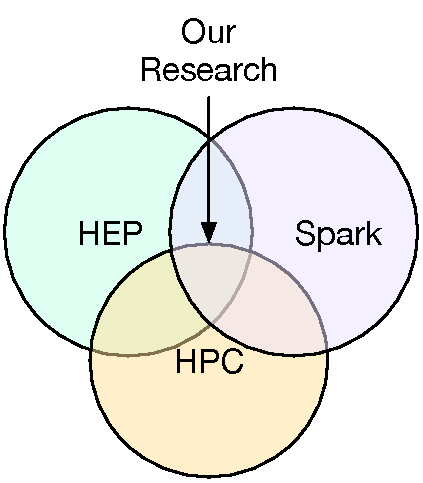
\includegraphics[scale=0.5]{overview}
\caption{The focus of our research}
\label{fig:overview}
\end{center}
\end{figure}
\squeezeup
